\documentclass[co342]{subfiles}

%% ========================================================
%% document

\begin{document}

    \chap{Planar Graphs} 

    \section{Planar Graphs}

    \begin{definition}{Planar}{Graph}
        Let $G$ be a graph.
        \begin{enumerate}
            \item A drawing of $G$ on a plane whose edges only intersect at common endpoints is called a \emph{planar embedding} of $G$.
            \item We say $G$ is \emph{planar} if there exists a planar embedding of $G$.
        \end{enumerate}
    \end{definition}

    \ex $K_4$ is a planar graph.
    \begin{eqbox}[A Planar Embedding of $K_4$]
        \begin{center}
            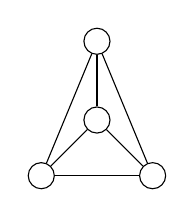
\begin{tikzpicture}[main/.style={draw,circle},node distance={1cm}]
                \node[main](0){};
                \node[main](1)[above of=0]{};
                \node[main](2)[below left of=0]{};
                \node[main](3)[below right of=0]{};
                \draw[-](0) -- (1);
                \draw[-](0) -- (2);
                \draw[-](0) -- (3);
                \draw[-](1) -- (2);
                \draw[-](1) -- (3);
                \draw[-](2) -- (3);
            \end{tikzpicture}
        \end{center}
    \end{eqbox} 
    
    \begin{definition}{Plane}{Graph}
        A \emph{plane} graph is a planar graph with a fixed planar embedding. We call vertices as \emph{points} and edges as \emph{lines}.
    \end{definition}
    
    \np A rigorous discussion of planarity involves topology, which is out of the scope of this note. But we shall take many topological results for granted. Moreover, we will mainly focus on the combinatorial aspects of planar graphs.

    \begin{recall}{Curve}{on a Topological Space}
        Let $X$ be a topological space. We say $C\subseteq X$ is a \emph{curve} on $X$ if there exists continuous $f:I\to X$ such that $C=\image\left( f \right)$, where $I\subseteq\R$ is an interval. We call $f$ a \emph{parameterization} of $C$.
    \end{recall}

    \begin{recall}{Simple, Closed, Jordan}{Curve}
        Let $C$ be a curve on a topological space $X$.
        \begin{enumerate}
            \item We say $C$ is \emph{simple} if it does not intersect itself, except at the endpoints.\footnote{Rigorously speaking, given a curve $C$ with a parameterization $f$ on an interval $I$, we say $C$ is simple if, for every $x,y\in I$, $f\left( x \right)=f\left( y \right)$ only if $x=y$ or $x,y$ are the endpoints of $I$.}
            \item We say $C$ is \emph{closed} if it is a continuous image of a unit circle.
            \item We say $C$ is \emph{Jordan} if $C$ is simple closed curve and $X=\R^{2}$.
        \end{enumerate}
    \end{recall}

    \begin{recall}{Connected}{Subset}
        Let $X$ be a topological space.
        \begin{enumerate}
            \item We say $X$ is \emph{disconnected} if $X$ is a union of two disjoint nonempty open subsets of $X$.
            \item We say $X$ is \emph{connected} if $X$ is not disconnected.
            \item A maximal connected subset of $X$ is called a \emph{connected component} of $X$.
        \end{enumerate}
    \end{recall}

    \begin{theorem}{Jordan Curve Theorem}
        Let $C$ be a Jordan curve. Then $\R^{2}\setminus C$ contains exactly $2$ connected components, one bounded and one unbounded.
    \end{theorem}

    \begin{recall}{Interior, Exterior}{of a Jordan Curve}
        Let $C$ be a Jordan curve.
        \begin{enumerate}
            \item The \emph{interior} of $C$, denoted as $\intr\left( C \right)$, is the bounded connected component of $\R^{2}\setminus C$.
            \item The \emph{exterior} of $C$, denoted as $\ext\left( C \right)$, is the unbounded connected component of $\R^{2}\setminus C$.
        \end{enumerate}
    \end{recall}

    \begin{cor}{}
        $K_5$ is not planar.
    \end{cor}

    \begin{proof}
        Suppose $K_5$ has a planar embedding for the sake of contradiction. Write $V\left( K_5 \right) = \left\lbrace v_1,v_2,v_3,v_4,v_5 \right\rbrace$. Then the lines
        \begin{equation*}
            v_1v_2,v_2v_3,v_3v_1
        \end{equation*}
        form a Jordan curve $C$, since $\left( \left\lbrace v_1,v_2,v_3 \right\rbrace, \left\lbrace v_1v_2,v_2v_3,v_3v_1 \right\rbrace \right)$ is a cycle in $K_5$. Then $v_4\in\intr\left( C \right)$ or $v_4\in\ext\left( C \right)$. Without loss of generality, assume $v_4\in\intr\left( C \right)$. Then the lines $v_4v_1,v_4v_2,v_4v_3$ are contained in $\intr\left( C \right)$, execpt at $v_1,v_2,v_3$, respectively. Let $C_1,C_2,C_3$ be the Jordan curves formed by the cycles
        \begin{equation*}
            \left( \left\lbrace v_2,v_3,v_4 \right\rbrace, \left\lbrace v_2v_3,v_3v_4,v_4v_2 \right\rbrace \right), \left( \left\lbrace v_1,v_3,v_4 \right\rbrace, \left\lbrace v_1v_3,v_3v_4,v_4v_1 \right\rbrace \right), \left( \left\lbrace v_1,v_2,v_4 \right\rbrace, \left\lbrace v_1v_2,v_2v_4,v_4v_1 \right\rbrace \right),
        \end{equation*}
        respectively. Note that, for all $i\in\left\lbrace 1,2,3 \right\rbrace$, $\intr\left( C_i \right)\subseteq\intr\left( C \right)$ and $v_i\in\ext\left( C \right)$. Since there is a line joining $v_5$ to $v_i$ for all $i\in\left\lbrace 1,2,3 \right\rbrace$, by the Jordan curve theorem $v_5\in\ext\left( C_i \right)$ for all $i\in\left\lbrace 1,2,3 \right\rbrace$. So $v_5\in\ext\left( C \right)$. But this contradicts the fact that $v_4\in\intr\left( C \right)$ and $v_4,v_5$ are joined by a line. Thus $K_5$ is not planar.
    \end{proof}

    \begin{cor}{}
        $K_{3,3}$ is not planar.
    \end{cor}

    \begin{definition}{Subdivision}{of a Graph}
        Let $G$ be a graph. A \emph{subdivision} of $G$ is obtained from $G$ by replacing each edge with a new path of length at least $1$.
    \end{definition}
    
    \begin{prop}{}
        Let $G$ be a graph. The following are equivalent.
        \begin{enumerate}
            \item $G$ is planar.
            \item Every subdivision of $G$ is planar.
        \end{enumerate}
    \end{prop}

    \begin{proof}[Proof-ish]
        Note that an edge and a path are both represented by a simple curve.
    \end{proof}

    \clearpage
    \begin{cor}{}
        Any graph containing a subdivision of $K_5$ or $K_{3,3}$ is not planar.
    \end{cor}	

    \section{Faces}
    
    \begin{definition}{Face}{of a Planar Embedding}
        A \emph{face} of a planar embedding is a maximal subset of points on the plane that are path-connected, and do not include any part of the embedding. The \emph{outer} face of an embedding is the unbounded face of the embedding. Each face is \emph{incident} to the vertices and edges on its boundary. We say two faces are \emph{adjacent} if they share at least one edge (or line) at their boundaries.
    \end{definition}

    \begin{prop}{}
        Let $f$ be a face of a plane graph $G$. Then there is an embedding of $G$ with the boundary of $f$ as the boundary of the outer face.
    \end{prop}

    \begin{prop}{}
        A graph can be embedded on a plane if and only if the graph can be embedded on a sphere.
    \end{prop}

    \begin{prop}{}
        Let $G$ be a plane graph. If $G$ is $2$-connected, then each face of $G$ is bounded by a cycle.\footnote{We say a face is \emph{bounded} by a cycle if its boundary is a cycle.}
    \end{prop}

    \begin{proof}
        There is an ear decomposition $\left( G_{i} \right)^{k}_{i=0}$ for $G$. We will treat each $G_i$ as the plane graph whose drawing is a part of the plane graph $G$. We will inductively prove that the result holds for each $G_i$. We see that $G_0$ is a cycle, so there are $2$ faces, each bounded by $G_0$. Suppose each face of $G_i$ is bounded by a cycle and further suppose $P_i$ is the ear such that $G_{i+1}=G_i+P_i$. Since $G_{i+1}$ is a plane graph, the curve representing $P_i$ must be entirely within a face $f$ of $G_i$ by the Jordan curve theorem. By induction, $f$ is bounded by a cycle, say $C$. The two endpoints of $P_i$ divides $C$ into $2$ paths $Q_1,Q_2$. Now $f$ is divided into $2$ faces, one bounded by $P_i+Q_1$ and the other bounded by $P_i+Q_2$, both of which are cycles. The remaining faces of $G_i$ are still faces of $G_{i+1}$, so they remain bounded by cycles. So the result holds for $G_{i+1}$. By induction, the result holds for $G_k=G$.
    \end{proof}

    \begin{cor}{}
        In a $3$-connected plane graph, all neighbors of a vertex lie on a common cycle.
    \end{cor}	
    
    \begin{proof}
        Let $G$ be a $3$-connected plane graph, and let $v\in V\left( G \right)$. Then $G-v$ is a $2$-connected plane graph. Moreover, the face $f$ of $G-v$ that contains $v$ is bounded by a cycle $C$ by Proposition 3.5. Since all neighbors of $v$ in $G$ lie on the boundary of $f$, they are on $C$.
    \end{proof}
    
    \begin{prop}{}
        The cycle space of a $2$-connected plane graph $G$ is spanned by the set of all facial cycles of $G$.\footnote{A cycle is called \emph{facial} if it is the boundary of a face.}
    \end{prop}

    \begin{proof}
        Any element of $\mC\left( G \right)$ is spanned by the cycles of $G$, so it suffices to show that each cycle is the sum of facial cycles. Let $C$ be any cycle, and let $S$ be the sum of all facial cycles of the faces inside $C$. Edges in the interior of $C$ are counted twice in $S$, once on each side. So they do not appear in $S$. On the other hand, edges on the cycle $C$ are counted once in $S$, as precisely one side is incide $C$. So $S=C$, as required.
    \end{proof}

    \begin{definition}{$2$-basis}{}
        Let $G$ be a graph. A \emph{$2$-basis} of a subspace of $\varep\left( G \right)$ is a basis $\beta$ where each edge of $G$ is in at most $2$ elements in $\beta$.
    \end{definition}

    \np It follows from Proposition 3.6 that every $2$-connected plane graph has a $2$-basis. We shall prove later that a graph is planar if and only if its cycle space has a $2$-basis, the result known as \textit{MacLane's theorem}.

    \section{Bridges}

    \begin{definition}{Bridge}{of a Subgraph}
        Let $H$ be a subgraph of a connected graph $G$. A \emph{bridge} of $H$ is
        \begin{enumerate}
            \item a component $J$ of $G-V\left( H \right)$ together with the edges in $\delta_G\left( V\left( J \right) \right)$ and their endpoints; or
            \item an edge not in $H$ that joins two vertices in $H$ (called a \emph{trivial} bridge).
        \end{enumerate}
    \end{definition}
    
    \begin{definition}{Vertex of Attachment (VOA)}{}
        Let $H$ be a subgraph of a connected graph $G$ and let $B$ be a bridge of $H$. A vertex $v$ of $B$ is called
        \begin{enumerate}
            \item a \emph{vertex of attachment} (\emph{VOA}) if $v$ is in $H$; and
            \item an \emph{internal} vertex if $v$ is not in $H$.
        \end{enumerate}
        We call a bridge with $k\in\N$ VOA a \emph{$k$-bridge}. We say two bridges are \emph{equivalent} if they have the same VOA.
    \end{definition}
    
    \begin{definition}{Segment}{}
        Let $C$ be a cycle. The $k$ VOA of a $k$-bridge partitions $C$ into $k$ \emph{segments}. 
        \begin{enumerate}
            \item Two bridges of $C$ \emph{avoid} each other if the VOA of one bridge are entirely within one segment of the other bridge. 
            \item Otherwise, we say they \emph{overlap}.
        \end{enumerate}
    \end{definition}

    \begin{definition}{Skew}{Bridges}
        Let $C$ be a cycle. We say two bridges of $C$ are \emph{skew} if there exists a sequence of distinct vertices $\left( v_{i} \right)^{4}_{i=1}$ on $C$ in cyclic order such that $v_1,v_3$ are VOA of one bridge and $v_2,v_4$ are VOA of the other bridge.
    \end{definition}
    
    \begin{prop}{}
        Overlapping bridges of a cycle are
        \begin{enumerate}
            \item skew; or
            \item equivalent $3$-bridges.
        \end{enumerate}
    \end{prop}

    \begin{proof}
        Let $B_1,B_2$ be two overlapping bridges of $C$. Then they both have at least $2$ VOA. Suppose $B_1,B_2$ are not equivalent. Then there must a VOA $u$ in $B_1$ but not in $B_2$. Suppose $u$ is in the segment $S$ for $B_2$, say from $x$ to $y$. Note that $x,u,y$ are distinct. Since $B_1,B_2$ overlap, there exists a VOA $v$ of $B_1$ that is not in $S$. Then $x,u,y,v$ are in cyclic order where $x,y$ are in $B_2$ and $u,v$ are in $B_1$. So $B_1,B_2$ are skew. On the other hand, suppose $B_1,B_2$ are are equivalent $k$-bridges. But equivalent $2$-bridges avoid each other, so $k\neq 2$. If $k=3$, then they are equivalent $3$-bridges. If $k\geq 4$, then they are skew by picking any $4$ VOA.
    \end{proof}

    \np Given a plane graph $G$ and a cycle $C$ in $G$, each bridge of $C$ is connected. By the Jordan curve theorem, each bridge is either intirely in $\overline{\intr\left( C \right)}$ or in $\overline{\ext\left( C \right)}$.

    \begin{definition}{Inner, Outer}{Bridge}
        Consider the setting of (3.4) and let $B$ be a bridge of $C$. We say $B$ is
        \begin{enumerate}
            \item \emph{inner} if $B\subseteq\overline{\intr\left( C \right)}$; and
            \item \emph{outer} if $B\subseteq\overline{\ext\left( C \right)}$.
        \end{enumerate}
    \end{definition}

    \begin{prop}{}
        Let $G$ be a plane graph. Then for every cycle $C$ of $G$,
        \begin{enumerate}
            \item inner bridges of $C$ avoid one another; and
            \item outer bridges of $C$ avoid one another.
        \end{enumerate}
    \end{prop}

    \noindent To prove Proposition 3.8, we introduce some notions and results.

    \begin{definition}{Branch}{Vertices of a Subdivision}
        A vertex in a subdivision is called \emph{branch} if its degree is at least $3$.
    \end{definition}

    \noindent We shall accept the following results without proof.

    \begin{fact}{}
        Let $C$ be a simple closed curve and let $p_1,\ldots,p_k\in C$ be distinct. Then for every $x\in\intr\left( C \right)$ ($y\in\ext\left( C \right)$), there are $k$ curves from $x$ to $p_i$'s such that
        \begin{enumerate}
            \item the curves are entirely in $\intr\left( C \right)$ ($\ext\left( C \right)$) except at $p_1,\ldots,p_k$; and
            \item they do not intersect each other except at $x$ ($y$).
        \end{enumerate}
    \end{fact}
    
    \begin{fact}{}
        Let $G$ be a connected graph and let $H$ be obtained from $G$ by adding $3$ distinct vertices $x_1,x_2,x_3$ and joining each $x_i$ to a vertex $v_i$ in $V\left( G \right)$. Then there exists $v\in V\left( G \right)$ such that there is a $3$-fan from $v$ to $\left\lbrace x_1,x_2,x_3 \right\rbrace$ in $H$.
    \end{fact}
    
    \begin{proof}[Proof-ish]
        First find a $v_1,v_2$-path and $v_1,v_3$-path in $G$. Let $v$ be the \textit{last} point of intersection and find a $3$-fan from there.
    \end{proof}
    
    \begin{proof}[Proof of Proposition 3.8]
        We shall prove (a) only, since a similar proof holds for (b). We first remove all outer bridges of $C$, so $C$ is the boundar of the outer face. Suppose, for the sake of contradiction, that there are overlapping inner bridges of $C$, say $B_1,B_2$. By Proposition 3.7, they are skew or equivalent $3$-bridges.
        \begin{itemize}
            \item \textit{Case 1. Suppose $B_1,B_2$ are skew.} Then there exist VOA $v_1,v_3$ in $B_1$ and $v_2,v_4$ in $B_2$ such that $v_1,v_2,v_3,v_4$ are distinct and in cyclic order on $C$. Since bridges are connected, there exists a $v_1,v_3$-path $p_1$ in $B_1$ and a $v_2,v_4$-path $P_2$ in $B_2$. Add a point $x$ in the $\ext\left( C \right)$, and use Fact 3.9 to draw curves from $x$ to $v_1,\ldots,v_4$ without intersecting. Treating $x$ as a vertex and each curve as an edge, we have a $4$-fan from $x$ to $\left\lbrace v_1,\ldots,v_4 \right\rbrace$ in $\overline{\ext\left( C \right)}$, and the resulting graph is plane. However, $\left\lbrace x,v_1,\ldots,v_4 \right\rbrace$ forms the branch vertices of a subdivision of $K_5$, by using the fan, the cycle $C$, and the two paths $P_1,P_2$. Hence the resulting graph is not planar, which is a contradiction. 
            \item \textit{Case 2. Suppose $B_1,B_2$ are equivalent $3$-bridges.} Let $v_1,v_2,v_3$ be the VOA for both bridges. Then by Fact 3.10, there are internal vertices $x_1,x_2$ in $B_1,B_2$, respectively, such that $3$-fans ffrom $x_1,x_2$ to $\left\lbrace v_1,v_2,v_3 \right\rbrace$ exist in $B_1,B_2$, respectively. Add a point $y$ in the $\ext\left( C \right)$, and use Fact 3.9 to draw a $3$-fan from $y$ to $\left\lbrace v_1,v_2,v_3 \right\rbrace$ without intersecting. The resulting graph is plane. However, the $3$-fans from $x_1,x_2,y$ to $v_1,v_2,v_3$ form a $K_{3,3}$ subdivision, using $v_1,v_2,v_3,x_1,x_2,y$ as branch vertices and the bipartition $\left\lbrace v_1,v_2,v_3 \right\rbrace, \left\lbrace x_1,x_2,y \right\rbrace$. But this means that the graph is not planar, a contradiction.
        \end{itemize} 
        Thus all inner bridges of $C$ avoid each other.
    \end{proof}

    \section{Kuratowski's Theorem}

    \begin{definition}{Kuratowski Subgraph (KS)}{}
        We call any subdivision of $K_5$ or $K_{3,3}$ a \emph{Kuratowski subgraph} (\emph{KS}).
    \end{definition}

    \begin{theorem}{Kuratowski's Theorem}
        A graph is planar if and only if it does not contain a Kuratowski subgraph.
    \end{theorem}

    \np[Proof Outline]The forward direction is provided by Corollary 3.2.1. Here is an outline for the reverse direction. We induct on the number of edges. Check base cases up to $6$ edges. Assume $G$ is not planar. The aim is to either find a KS or reach a contradiction (i.e. showing that $G$ is planar).
    \begin{enumerate}
        \item $G$ is not planar if and only if a component of $G$ is not planar. So we may assume $G$ is connected.
        \item The case when $G$ has a cut-vertex is easy. Apply induction to each \textit{component} to either find a KS or find an embedding around the cut-vertex.
        \item The case when $G$ has a separating set of size $2$ is not hard. Apply induction to each \textit{component}.
        \item Assume $G$ is $3$-connected. Then there exists an edge where $G /e$ is $3$-connected.
            \begin{enumerate}
                \item If $G /e$ is not planar, t hen it has a KS by induction. \textit{Uncontract} $e$ to find a KS for $G$.
                \item If $G /e$ is planar, then there is a planar embedding. We look at the cycle around the neighbors of the contracted vertex. When we \textit{uncontract} $e$, we look at how the neighbors of the two ends of $e$ land on the cycle. If they do not overlap, then we can find a planar embedding for $G$. If they do overlap, then we can find a KS.
            \end{enumerate}
    \end{enumerate}
    \noindent Before we move on to the proof of Kuratowski's theorem, here are some results that we are going to utilize for the proof of Kuratowski's theorem.
    
    \begin{lemma_inside}{}
        Suppose $G$ is a plane graph and $C$ is a simple closed curve. Then
            \begin{enumerate}
                \item we can embed $G$ into $\intr\left( C \right)$;
                \item if we pick a point $v$ in the outer face of $G$ and a point $x$ on $C$, then we can embed $G$ into $\overline{\intr\left( C \right)}$ where $v=x$; and
                \item if we pick a line $uw$ on the outer face of $G$ and a curve joining $y,z$ on $C$, then we can embed $G$ into $\overline{\intr\left( C \right)}$ where $uw$ is the curve from $y$ to $z$.
            \end{enumerate}
    \end{lemma_inside}

    \noindent We also have a result from connectivity regarding minimal separating sets.

    \clearpage
    \begin{lemma_inside}{}
        If $X$ is a minimal separating set of $G$, then every vertex in $X$ is adjacent to at least one vertex in each component of $G-X$.
    \end{lemma_inside}

    \begin{proof}[Proof of Kuratowski's Theorem]
        We prove the backward direction only, as Corollary 3.2.1 provides the forward direction. 

        We proceed by the induction on the number of edges. We can manually check that any graph with at most $6$ edges is planar.

        Now assume that $G$ is a nonplanar graph with at least $7$ edges, where we desire to find a Kuratowski subgraph in $G$. We break down the proof into few cases. We may assume that $G$ is connected, since at least one component of $G$ is nonplanar.
        \begin{itemize}
            \item \textit{Case 1. Suppose $G$ has a cut vertex, say $v$.} Let $H_1,\ldots,H_k$ be the bridges of $v$. That is, $G-v$ has many components, and we add $v$ (and adjacent edges) to each component to form $H_1,\ldots,H_k$. Since there are at least $2$ components in $G-v$, each bridge $H_i$ has fewer edges than $G$. 

                We now claim that at least one of $H_1,\ldots,H_k$ is nonplanar. For the sake of contradiction, assume every $H_i$ is planar. For each $H_i$, find an embedding where $v$ on the outer face (i.e. find a face containing $v$, and use Proposition 3.3). We now find an embedding of $G$ as follows. Place $v$ anywhere on the plane. Partition a neighborhood of $v$ into $k$ \textit{slices}, and embed each $H_i$ to a distinct slice, making sure that $v$ is the same point for each embedding. But this means $G$ is planar, a contradiction.

                Hence we can find nonplanar $H_i$, and by induction $H_i$ has a Kuratowski subgraph. Thus $G$ contains a Kuratowski subgraph.

            \item \textit{Case 2. Suppose $G$ is $2$-connected.} Let $S$ be a separating set of $G$ of size $2$ and let $H_1,\ldots,H_k$ be the bridges of $S$ together with edge $xy$ (even if $xy$ is not an edge in $G$). Since $S$ is a minimal separating set, both $x,y$ are adjacent to some vertices in each component of $G-S$.

                Suppose $H_i$ is not planar for some $i$. Note $H_i$ has fewer edges than $G$. By induction, $H_i$ has a Kuratowski subgraph, say $J$. If $J$ does not contain $xy$, then we are done. Otherwise, there is an $x,y$-path $P$ through a different bridge. We can replace $xy$ with $P$ in $J$ to get a Kuratowski subgraph in $G$.

                On the other hand, assume every $H_i$ is planar for the sake of contradiction. Then there exists an embedding of each $H_i$ with $xy$ on the outer face. We now construct an embedding of $G$ inductively. Start with an embedding of $H_1$. Suppose we have embedded $H_1,\ldots,H_i$. We look for a face containing $xy$, and embed $H_{i+1}$ in this face. Once we embed $H_k$, remove $xy$ if it is not in $G$. This means $G$ is planar, a contradiction.

            \item \textit{Case 3. Suppose $G$ is $3$-connected.} There exists $e=xy$ in $G$ such that $G /e$ is $3$-conencted. Let $z$ be the contracted vertex. We break into 2 cases.
                \begin{itemize}
                    \item \textit{Case 3.1. Suppose $G /e$ is not planar.} By induction, $G /e$ contains a Kuratowski subgraph $H$. If $H$ does not contain $z$, then $H$ is a Kuratowski subgraph of $G$. We now suppose $z$ is in $H$. 

                        Suppose $z$ is not a branch vertex (i.e. $\deg_H\left( z \right)=2$). Let $u,v$ be the two neighbors of $z$ in $H$. When we \textit{uncontract} $e$, both $u,v$ are adjacent to at least one of $x,y$. If both $u,v$ are adjacent to the same vertex, say without loss of generality $x$, then we can replace the path $\left( u,z,v \right)$ by $\left( u,x,v \right)$. If $u,v$ are adjacent to different vertices, say $ux, vy$ are edges, then we can replace the path $\left( u,z,v \right)$ by $\left( u,x,y,v \right)$. In either case, we have found a Kuratowski subgraph in $G$.

                        Suppose $z$ is a branch vertex. Let $S$ be the set of all neighbors of $z$ in $H$. WHen we \textit{uncontract} $e$, each vertex in $S$ is adjacent to at least one of $x,y$. If $x$ is adjacent to all vertices in $S$, then we can replace $z$ with $x$ to obtain a Kuratowski subgraph for $G$. Similar result holds when $y$ is adjacent to all vertices in $S$. Suppose $x$ is adjacent to all but one vertex in $S$, say $w$. Then $y$ is adjacent to $w$. So we can replace $z$ with $x$ as the new branch vertex, and replace $zw$ with the path $\left( x,y,w \right)$. This gives a Kuratowski subgraph in $G$. Finally, when both $x,y$ are adjacent to $2$ vertices in $S$, and they are distinct. Then $H$ is a subdivision of $K_5$. Let $w_1,\ldots,w_4$ be the other $4$ branch vertices. Suppose without loss of generality the two neighbors of $x$ are on the $z,w_1$-path, $z,w_2$-path in $H$, and the two neighbors of $y$ are in $z,w_3$-path, $z,w_4$-path. Then there is a subdivision $K{3,3}$ with $\left\lbrace x,w_3,w_4 \right\rbrace, \left\lbrace y,w_1,w_2 \right\rbrace$ as the bipartition of the branch vertices. This is a Kuratowski subgraph in $G$.

                    \item \textit{Case 3.2. Suppose $G /e$ is planar.} Since $G /e$ is $3$-connected, the neighbors of $z$ are in a cycle $C$. When we \textit{uncontract} $e$, each such vertex is adjacent to at least one of $x,y$. Let $H_x, H_y$  be the bridges of $C$ in $G-xy$ containing $x,y$, respectively. Note that everything outside $C$ is still planar.

                        Suppose $H_x,H_y$ avoid each other. First draw $H_x$ in $C$: place $x$ in $\intr\left( C \right)$ and add nonintersecting lines to the neighbors of $x$. Then the VOA of $H_y$ are within one segment $P$ of $H_x$, say it is from $u$ to $v$. Then $P+vx,xu$ form the boundary of a face. We then embed $H_y$ and $xy$ inside this face. This is a planar embedding of $G$, which is a contradiction. Hence $H_x, H_y$ overlap.

                        Since $H_x,H_y$ overlap, they are skew or equivalent $3$-bridges.

                        Suppose $H_x, H_y$ are skew. Then there exist vertices $x_1,y_1,x_2,y_2$ in cyclic order on $C$ such that $x_1,x_2$ are in $H_x$, $y_1,y_2$ are in $H_y$. Then there is a $K_{3,3}$ subdivision in $C\cup\left\lbrace xx_1,xx_2,yy_1,yy_2,xy \right\rbrace$ with $\left\lbrace x_1,y_1,y_2 \right\rbrace , \left\lbrace y,x_1,x_2 \right\rbrace$ as the bipartition of the brach vvertices. This is a Kuratowski subgraph in $G$.

                        Suppose $H_x, H_y$ are equivalent $3$-bridges, with $w_1,w_2,w_3$ as their common VOA. Then $C\cup H_x\cup H_y\cup \left\lbrace xy \right\rbrace$ is a subdivision of $K_5$ with $\left\lbrace x,y,w_1,w_2,w_3 \right\rbrace$ as the branch vertices. This is a Kuratowski subgraph in $G$. \qqedsym
                \end{itemize} 
        \end{itemize} 
    \end{proof}
    
    \section{Wagner's Theorem}
    
    \begin{definition}{Minor}{of a Graph}
        Let $G$ be a graph. We say a graph $H$ is a \emph{minor} of $G$ if $H$ can be obtained from $G$ by a series of vertex and edge deletions, and edge contractions.
    \end{definition}

    \np Each vertex in the minor is a result of a series of edge contractoins (possibly none), and the vertices involved must be connected. Another way to think about a minor is the following. First partition the vertices of $G$ into $V_0,\ldots,V_k$ where $G\left[ V_i \right]$ is connected for each $i\in\left\lbrace 1,\ldots,k \right\rbrace$. We then delete $k_0$, and shrink $V_1,\ldots,V_k$ into $k$ vertices.

    \begin{prop}{}
        Let $G$ be a graph. If $G$ has a subdivision of $H$, then $H$ is a minor of $G$.
    \end{prop}

    \begin{theorem}{Wagner's Theorem}
        A graph $G$ is planar if and only if $G$ does not have $K_5$ or $K_{3,3}$ as a minor.
    \end{theorem}
    
    \begin{prop}{}
        A graph $G$ contains a subdivision of $K_5$ or $K_{3,3}$ if and only if $G$ has $K_5$ or $K_{3,3}$ as a minor.
    \end{prop}

    \begin{proof}
        The forward direction is provided by Proposition 3.12. Suppose that $G$ has $K_5$ or $K_{3,3}$ as a minor.
        \begin{itemize}
            \item \textit{Case 1. Suppose $G$ has $K_{3,3}$ as a minor.} So there is a subgraph of $G$ where the vertices can be partitioned into $A_1,A_2,A_3,B_1,B_2,B_3$ such that each induces a connected subgraph, and shrinking all $6$ sets results in a $K_{3,3}$. In $G$, between each pair $A_i,B_j$, there is an edge joining a vertex of $A_i$ with a vertex of $B_j$. Since each $A_i, B_j$ induces a connected subgraph, there exists a $3$-fan from some vertex in each $A_i, B_j$ to the $3$ endpoints. These fans form a subdivision of $K_{3,3}$.

            \item \textit{Case 2. Suppose $G$ has $K_5$ as a minor.} We sketch the proof only. The $5$ branch vertices correspond to $5$ sets of vertices that induce connected subgraphs. There are edges between each set. If an appropriate $4$-fan exists in all $5$ sets, then we have a $K_5$ subdivision. Otherwise, we find some $3$-fan in one set. Find an internally disjoint path from the fan to the $4$th vertex. We can find appropiarte $3$-fans from the other $4$ sets, and this gives a $K_{3,3}$ subdivision. \qqedsym
        \end{itemize} 
    \end{proof}
    
    \begin{theorem}{Graph Minor Theorem}
        Any infinite sequence $\left( G_{i} \right)^{\infty}_{i=1}$ of finite graphs includes two graphs $i,j$ with $i<j$ such that $G_i$ is a minor of $G_j$.
    \end{theorem}

    \begin{proof}
        Tl;dr.
    \end{proof}

    \begin{definition}{Minor-closed}{Collection of Graphs}
        We say a collection $\mG$ of graphs is \emph{minor-closed} if any minor of any graph in $\mG$ is also in $\mG$.
    \end{definition}

    \ex
    \begin{enumerate}
        \item The collection of planar graphs is minor-closed.
        \item More generally, any collection of all graphs that can be embedded on a particular surface is minor-closed.
        \item The collection of all forests is minor closed.
    \end{enumerate}
    
    \begin{definition}{Minor-minimal}{Graph}
        A graph $G$ is \emph{minor-minimal} in a minor-closed collection of graphs $\mG$ if $G\notin\mG$ but any proper minor of $G$ is in $\mG$.
    \end{definition}

    \ex By Wagner's theorem, the only minor-minimal graphs for the collection of planar graphs are $K_5, K_{3,3}$. We sometimes call $K_5, K_{3,3}$ the \textit{forbidden minors}.
    
    \begin{prop}{}
        For any minor-closed collection of graphs $\mG$, there is a finite number of minor-minimal graphs.
    \end{prop}

    \begin{proof}
        Suppose there are infinitely many minor-minimal graphs, for the sake of contradiction. By the graph minor theorme, there exists two such graphs $G,H$ such that $G$ is a minor of $H$, contradicting the fact that $H$ is minor-minimal.
    \end{proof}
    
    \np Proposition 3.16 implies that, given any surface $S$, there exists a finite collection of graphs $\mG$ where \textit{$G$ can be embedded in $S$ if and only if $G$ does not contain any graph in $H$ as a minor.} For the torus, we do not exactly know what $\mG$ is, but we at least know $16000$ forbidden minors. One should also note that we cannot generalize Kuratowski's theorem in an analogous way; if we replace \textit{minor} with \textit{subdivision} above, then it is false in general.
    
    \section{MacLane's Theorem}

    \begin{recall}{$2$-basis}{}
        Let $G$ be a graph. A \emph{$2$-basis} of a subspace of $\varep\left( G \right)$ is a basis $\beta$ where each edge of $G$ is in at most $2$ elements in $\beta$.
    \end{recall}

    \begin{theorem}{MacLane's Theorem}
        A graph $G$ is planar if and only if the cycle space of $G$ has a $2$-basis.
    \end{theorem}

    \np[Main Idea for the Backward Direction]If $G$ is not planar, then we can use deletions and contractions to get $K_5$ or $K_{3,3}$. We show that if $\mC\left( G \right)$ has a $2$-basis, then any deletion or contraction results in a graph whose cycle space has a $2$-basis. Finally, we show that $\mC\left( K_5 \right),\mC\left( K_{3,3} \right)$ do not have $2$-bases. We prove each step as a separate proposition.

    \begin{prop}{}
        If $H$ is a minor of $G$ and $\mC\left( G \right)$ has a $2$-basis, then $\mC\left( H \right)$ has a $2$-basis.
    \end{prop}

    \begin{proof}[Proof Sketch]
        Suppose $G_0,\ldots,G_m$ is a sequence of graphs where $G_0=G, G_m=H$, and $G_{i+1}$ can be obtained from $G_i$ by removing an isolated vertex, removing an edge, or contracting an edge. Note that deleting a vertex is equivalent to removing all edges incident with it and then removing the isolated vertex. We prove by induction that $\mC\left( G_i \right)$ has a $2$-basis for each $i$. By assumption, $G_0=G$ has a $2$-basis.

        We now assume $i\geq 1$. Suppose $G_i$ has $c$ components, and $\left\lbrace E_1,..,E_k \right\rbrace$ is a $2$-basis of $\mC\left( G_i \right)$, where
        \begin{equation*}
            k = \left| E\left( G_i \right) \right|-\left| V\left( G_i \right) \right|+c.
        \end{equation*}
        We now break into $3$ cases.
        \begin{itemize}
            \item \textit{Case 1. Suppose $G_{i+1}$ is obtianed from $G_i$ by removing an isolated vertex.} Then $E\left( G_{i+1} \right)=E\left( G_i \right)$, so all edges in $\left\lbrace E_1,\ldots,E_k \right\rbrace$ are still in $G_{i+1}$. Also, $G_{i+1}$ has one fewer vertex and component than $G$, so
                \begin{equation*}
                    \dim\left( \mC\left( G_{i=1} \right) \right) = \left| E\left( G_{i+1} \right) \right| - \left( \left| V\left( G_i \right) \right|-1 \right)+\left( c-1 \right) = \left| E\left( G_i \right) \right|-\left| V\left( G_i \right) \right|+c = k.
                \end{equation*}
                Since $\left\lbrace E_1,\ldots,E_k \right\rbrace$ is independent with $\dim\left( \mC\left( G_{i+1} \right) \right)$ elements, it is a basis of $\mC\left( G_{i+1} \right)$. Hence $\left\lbrace E_1,\ldots,E_k \right\rbrace$ is a $2$-basis for $\mC\left( G_{i+1} \right)$.

            \item \textit{Case 2. Suppose $G_{i+1}$ is obtained from $G_i$ by removing an edge $e$.} If $e$ is a cut-edge, then $e$ is not in any cycle. This means $\left\lbrace E_1,\ldots,E_k \right\rbrace$ is still a basis for $\mC\left( G_{i+1} \right)$ and the result follows. 

                On the other hand, suppose $e$ is not a cut-edge. Then $e$ is in $1$ or $2$ elements of $\left\lbrace E_1,\ldots,E_k \right\rbrace$. Suppose $e$ is in exactly $1$ element, say without loss of generality $E_k$. Then $\left\lbrace E_1,\ldots,E_{k-1} \right\rbrace$ is a $2$-basis for $\mC\left( G_{i+1} \right)$ and the resultt follows.

                Now assume $e$ is in two elements, say without loss of generality $E_{k-1}, E_k$. Then $\left\lbrace E_1,\ldots,E_{k-2},E_{k-1}+E_k \right\rbrace$ is a $2$-basis for $\mC\left( G_{i+1} \right)$.

            \item \textit{Case 3. Suppose $G_{i+1}$ is obtained from $G_i$ by contracting an edge $e$.} Consider $\left\lbrace E_1-e,\ldots,E_k-e \right\rbrace$. Note that if $z$ is the contracted vertex and $e=uv$, then 
                \begin{equation*}
                    \deg_{E_j-e}\left( z \right) = \deg_{E_j}\left( u \right)+\deg_{E_j}\left( v \right)-2,
                \end{equation*}
                which is still even. So $E_j-e$ is even. Then $\left\lbrace E_1-e,\ldots,E_k-e \right\rbrace$ is a $2$ basis for $\mC\left( G_{i+1} \right)$. \qqedsym
        \end{itemize} 
    \end{proof}
    
    \clearpage
    \begin{prop}{}
        $\mC\left( K_5 \right),\mC\left( K_{3,3} \right)$ do not have $2$-bases. 
    \end{prop}

    \begin{proof}
        Suppose $\mC\left( K_5 \right)$ has a $2$-basis for the sake of contradiction. We see that $\dim\left( \mC\left( K_5 \right) \right)=10-5+1=6$. So suppose $\left\lbrace E_1,\ldots,E_6 \right\rbrace$ is a $2$-basis for $\mC\left( K_5 \right)$. Let
        \begin{equation*}
            E_7 = \sum^{6}_{i=1}E_i.
        \end{equation*}
        Since $\left\lbrace E_1,\ldots,E_6 \right\rbrace$ is independent, $E_7$ is not empty. In fact, $E_7$ contains all the edges that appear in $E_1,\ldots,E_6$ exactly once. So $\left\lbrace E_1,\ldots,E_7 \right\rbrace$ contains each edge exactly twice. Since $K_5$ has $10$ edges, they appear in $\left\lbrace E_1,\ldots,E_7 \right\rbrace$ $20$ times in total. By pigenhole principle, at least one element $E_i$ has at most $2$ edges. However, each element is nonempty, and must contain at least one cycle, which has at least $3$ edges. This is a contradiction.

        The case for $\mC\left( K_{3,3} \right)$ is left as an exercise.
    \end{proof}

    \begin{proof}[Proof of MacLane's Theorem]
        \begin{itemize}
            \item ($\implies$) Suppose $G$ is planar. Then each block of $G$ is planar. Then we can show that $\mC\left( G \right)$ has a $2$-basis if and only if the cycle space of each of its blocks has a $2$-basis. If a block consists of only $1$ edge, then its cycle space is the trivial subspace, so it has a $2$-basis. If a block $B$ is $2$-connected, then in an embedding of $B$, its facial cycles span $\mC\left( B \right)$. Every edge is in $2$ facial cycles, so a subset of the facial cycles is a $2$-basis for $\mC\left( B \right)$.

            \item ($\impliedby$) Suppose $G$ is not planar. By Wagner's theorem, $G$ has $K_5$ or $K_{3,3}$ as a minor. it follows from Proposition 3.18, 3.19 that $\mC\left( G \right)$ does not have a $2$-basis. \qqedsym
        \end{itemize} 
    \end{proof}

    \section{Dual Graphs}
    
    \np We discuss dual graphs and their results without proof.

    \begin{definition}{Dual}{of a Plane Graph}
        Let $G$ be a graph. We define the \emph{dual} of $G$, denoted as $G^{*}$, as follows. Each face $f$ of $G$ corresponds to a vertex $f^{*}$ in $G^{*}$; for each edge $e$ in $G$ with faces $f,g$ on its two sides, there is a corresponding edge $e^{*}=f^{*}g^{*}$.
    \end{definition}

    \noindent Note that by definition, even if $G$ is simple, $G^{*}$ can have multiple edges and loops.
    \begin{enumerate}
        \item Multiple edges appaer when several edges have the same faces on both sides.
        \item Loops appear when the two sides of an edge are in the same face.
    \end{enumerate}

    \begin{prop}{}
        If $G$ is a plane graph, then $G^{*}$ is a plane graph.
    \end{prop}

    \np[Proof Idea for Proposition 3.20]Given a plane graph, place a point in the interior of each face to represent the dual vertices. Then find \textit{fans} to the midpoints of the edges on its boundary. For each edge, join the lines on both sides to form corresponding dual edges.
    
    \clearpage
    \begin{prop}{}
        For any plane graph $G$, $G^{*}$ is connected.
    \end{prop}

    \np[Proof Idea for Proposition 3.21]Given a plane graph, take any two face vertices. Join them with any arbitrary curve. Trace the sequence of faces visited in the curve to find a walk in the dual.

    \begin{cor}{}
        If $G$ is a connected plane graph, then $\left( G^{*} \right)^{*}=G$.
    \end{cor}	
    
    \begin{prop}{}
        Let $G$ be a conected plane graph and let $e$ be an edge. 
        \begin{enumerate}
            \item If $e$ is not a cut-edge, then $\left( G-e \right)^{*} = G^{*} /e^{*}$.
            \item If $e$ is not a loop, then $\left( G /e \right)^{*} = G^{*}-e^{*}$.
        \end{enumerate}
    \end{prop}
    
    \begin{prop}{}
        Let $G$ be a connected plane graph.
        \begin{enumerate}
            \item If $C$ is a cycle in $G$, then $C^{*}=\left\lbrace e^{*}:e\in C \right\rbrace$ is a bond in $G^{*}$.
            \item If $B$ is a bond in $G$, then $B^{*}=\left\lbrace e^{*}:e\in B \right\rbrace$ is a bond in $G^{*}$.
        \end{enumerate}
    \end{prop}
    
    \begin{cor}{}
        For a connected plane graph $G$, $\mC\left( G \right)=\mC^{*}\left( G^{*} \right)$ and $\mC^{*}\left( G \right)=\mC\left( G^{*} \right)$.\footnote{We are \textit{treating} $e,e^{*}$ as the \textit{same} element.}
    \end{cor}	

    \np Proposition 3.23 motivates the following definition.
    
    \begin{definition}{Abstract Dual}{}
        Let $G,G^{*}$ be two graphs with the same edge sets. We say $G,G^{*}$ are \emph{abstract duals} if the set of all cycles in $G$ is the same as the set of all bonds in $G^{*}$, and the set of all bonds in $G$ is the same as the set of all cycles in $G^{*}$.
    \end{definition}
    
    \np If $G$ is a connected plane graph, then $G,G^{*}$ are abstract duals.

    \begin{prop}{}
        If $G,G^{*}$ are connected abstract duals, then $\mC\left( G \right)=\mC^{*}\left( G^{*} \right), \mC^{*}\left( G \right)=\mC\left( G^{*} \right)$.
    \end{prop}
    
    \begin{theorem}{Whitney's Theorem}
        A connected graph $G$ is planar if and only if $G$ has an abstract dual.
    \end{theorem}
    
    \begin{proof}
        If $G$ is planar, then its plane dual $G^{*}$ is its abstract dual. Conversely, suppose $G$ has an abstract dual $G^{*}$. Then $\mC\left( G \right)=\mC^{*}\left( G^{*} \right)$. Now we can show that $\left\lbrace \delta\left( \left\lbrace v \right\rbrace \right) \right\rbrace^{}_{v\in V\left( G^{*} \right)}$ spans $\mC^{*}\left( G^{*} \right)$. Moreover, each edge $e=uv$ is in two elements in the set: $\delta\left( \left\lbrace u \right\rbrace \right),\delta\left( \left\lbrace v \right\rbrace \right)$. Hence a subset of $\left\lbrace \delta\left( \left\lbrace v \right\rbrace \right) \right\rbrace_{v\in V\left( G^{*} \right)}$ is a  $2$-basis for $\mC^{*}\left( G^{*} \right)$. But $\mC^{*}\left( G^{*} \right)=\mC\left( G \right)$, so we have a $2$-basis for $\mC\left( G \right)$. Thus by MacLane's theorem, $G$ is planar.
    \end{proof}
    
    
    
    
    
    
    
    
    
    
    
    
    
    
    
    
    
    
    
    
    
    
    
    


















\end{document}
